\begin{figure}[t]
	\begin{center}
		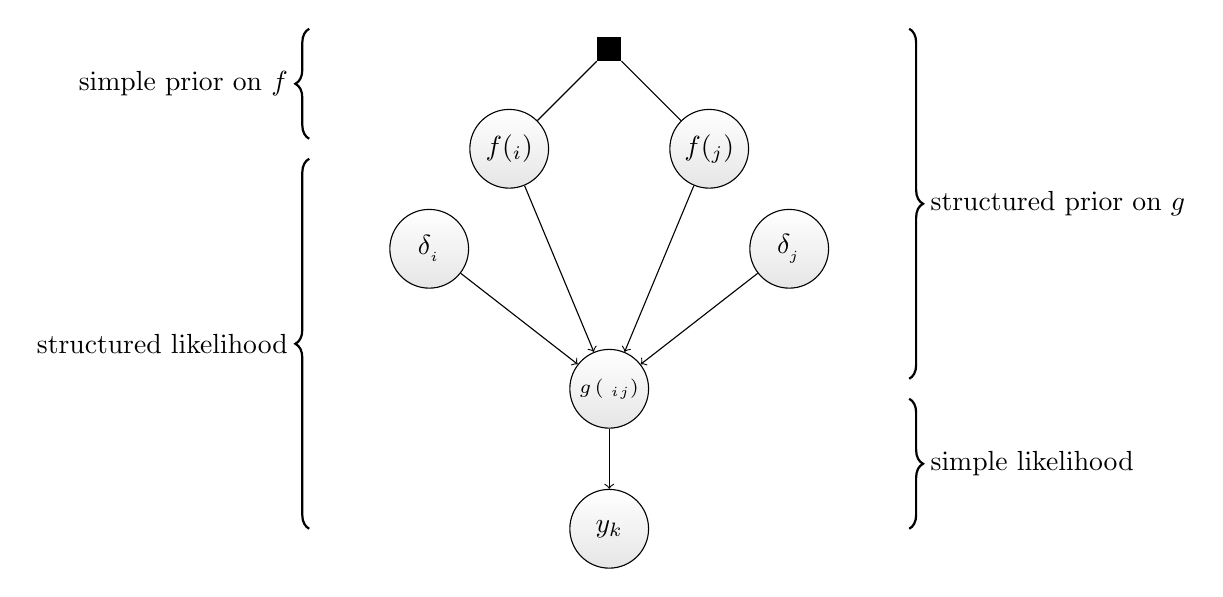
\begin{tikzpicture}
				\node at (2.5in,2.4in) [fill =black, rectangle,inner sep=0pt, minimum size = 0.3cm] (factor) {};
				\node at (2in,1.9in) [draw, circle,inner sep=0pt, minimum size = 1cm, top color=white, bottom color=black!10] (f_1) {$f(\x_i)$};
				\node at (3in,1.9in) [draw, circle,inner sep=0pt, minimum size = 1cm, top color=white, bottom color=black!10] (f_2) {$f(\x_j)$};
				\node at (1.6in,1.4in) [draw, circle,inner sep=0pt, minimum size = 1cm, top color=white, bottom color=black!10] (delta_2) {$\delta_{\x_i}$};	
				\node at (3.4in,1.4in) [draw, circle,inner sep=0pt, minimum size = 1cm, top color=white, bottom color=black!10] (delta_1) {$\delta_{\x_j}$};
				\node at (2.5in,0.7in) [draw, circle,inner sep=0pt, minimum size = 1cm, top color=white, bottom color=black!10] (g) {\scriptsize $g\left(\begin{matrix}\x_i\\\x_j\\\end{matrix}\right)$};
				\node at (2.5in,0in) [draw, circle,inner sep=0pt, minimum size = 1cm, top color=white, bottom color=black!10] (y) {$y_k$};
				\draw [->] (g) to (y);
				\draw  (factor) to (f_1);
				\draw (factor) to (f_2);
				\draw [->] (f_1) to (g);			
				\draw [->] (f_2) to (g);
				\draw [->] (delta_1) to (g);
				\draw [->] (delta_2) to (g);
				\draw [thick,decorate,decoration={brace,amplitude=5pt},] (1in,1.95in)  -- (1in,2.5in)
					node [black,midway,left=4pt] {simple prior on $f$};
				\draw [thick,decorate,decoration={brace,amplitude=5pt}] (1in,0in)  -- (1in,1.85in)
					node [black,midway,left=4pt] {structured likelihood};
				\draw [thick,decorate,decoration={brace,amplitude=5pt}] (4in,2.5in)  -- (4in,0.75in)
									node [black,midway,right=4pt] {structured prior on $g$};
				\draw [thick,decorate,decoration={brace,amplitude=5pt}] (4in,0.65in)  -- (4in,0in)
					node [black,midway,right=4pt] {simple likelihood};
			\end{tikzpicture}
	\end{center}
		\caption{Generative model underlying the preference learning framework. \emph{Left:} the original approach \citep{chu2005} considers the latent preference function $f$ as latent parameter, and the rest of the graphical model as a complex, structured likelihood. \emph{Right:} Our approach re-parametrises the problem in terms of $g$, and thus works with a simpler likelihood but with a more structured prior. The prior takes the form of a Gaussian Process with the preference judgement covariance function. \label{fig:graphical_model}}
\end{figure}
